\section{Discussion}

Looking at the results, the interaction were various depending on the plant. Thus, we can extract main interactions that are linked to the plant type. Looking at tab. \ref{tab:results}, people are more inclined to use their hands as tam tam or grasp the \textit{Pachira glabra}. However, for the \textit{Dracaena} people prefer to pinch the trunk or leave. People decided to grasp whether a pack of trunk or leaves when it came to \textit{Dypsis lutescens}.
This is induced by many factors including the leaves shape, the width of the trunk.


It was observed that when the plants were positioned at higher elevations on the table, individuals tended to engage more with the trunk of the plants. \hl{link to the future graph}

Looking at table \ref{tab:results}, we decided to group interaction. This was done by grouping type of interaction depending on 3 main factors :

\begin{itemize}
    \item The intensity factor : what is the intensity of the interaction (ex : pinch is lighter than grasp)
    \item The spatial factor : what is the interaction displacement.
    \item The duration factor : what is the interaction duration (ex : tam tam is instantaneous).
\end{itemize}

The "Group 1" includes the pinch and grasp interaction. Indeed, looking at the 3 factors we defined, the pinch and grasp are high in intensity and long in duration but people stay still in space.

The "Group 2" includes the slide. The slide interaction is long in time, it moves in space but low in intensity.

Whereas, the "Group 3" includes the pet and Tam Tam. These 2 interactions are really high in intensity, people usually tam tam and pet in different places but those interactions are short in time. 


\begin{figure}[h]
    \centering
    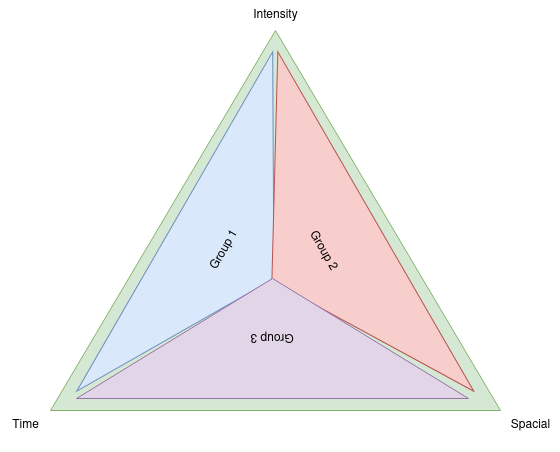
\includegraphics[width=0.42\textwidth]{Images/iop_triangle.png}
    \caption{Graph that is allowing to visualize the possible extracted properties of interactions types. Group 1, 2 and 3 refers to the group in the table \ref{tab:results}.}
    
    \vspace{-0.5cm}
    \label{fig:interaction_type_triangle}
    \vspace{0.2cm}
\end{figure}


%\hl{add 3D graph}